\documentclass[10pt,letterpaper]{article}
% \documentclass[stu,12pt,floatsintext]{apa7}
\usepackage{geometry,
  multicol,
  graphicx,
  verbatim,
  fancyhdr,
  lipsum,
  lineno,
  blindtext,
  wrapfig,
  authblk,
  hyperref,
  csquotes
}
\usepackage[american]{babel}

\providecommand{\tightlist}{%
  \setlength{\itemsep}{0pt}\setlength{\parskip}{0pt}}

\author[1]{Calypsa McCarthy}
\author[2]{Salma Ouaakki}
\author[3]{Noah Jones}
\affil[1]{\href{mailto:cmccarthy3@ufl.edu}{cmccarthy3@ufl.edu}\\University of Florida, Institute of Food and Agricultural Sciences}
\affil[2]{\href{mailto:salma.ouaakki@ufl.edu}{salma.ouaakki@ufl.edu}\\University of Florida, Herbert Wertheim College of Engineering}
\affil[3]{\href{mailto:noahtjones@ufl.edu}{noahtjones@ufl.edu}\\(Mentor) University of Florida, College of Medicine}
\date{March 2024}

\title{A Functional and Statically Typed Framework for Correctness and Scalability Implemented in Haskell}
% \shorttitle{Haskell Bioinformatics Framework}
% \author{Calypsa McCarthy and Salma Ouaakki}
% \professor{Noah Jones}
% \duedate{March 15, 2024}
% \affiliation{University of Florida}
% \course{Undergraduate High-performance Computing Scholarship}

\usepackage[backend=biber,style=apa,sorting=nyt]{biblatex} %Imports biblatex package
\DeclareLanguageMapping{american}{american-apa}
\addbibresource{bibliography.bib} %Import the bibliography file

% Discuss testing the pipeline against some standard dataset/pipeline

\begin{document}
% \linenumbers
\maketitle

\begin{abstract}
  There is a growing preponderance of high-dimensional data sets
  across various research fields, posing challenges related to the
  limitations of current analysis tools. Shortcomings of
  parallelizability, concurrency, and the integration of disparate
  data types have been widely acknowledged. Despite the
  prevalence of dimensionality reduction techniques in machine
  learning, a distributed version of one of the most popular
  algorithms, uniform manifold approximation and projection (UMAP),
  remains unavailable thus hindering the scalability of data
  pipelines and workflows. Additionally, while statistical analysis
  methods like R and Java are commonly used among bioinformatics
  researchers, there lacks a commercial or open-source core
  framework with features emphasizing reliability, type safety, and
  correctness guarantees.

  To address these challenges, this project proposes the development
  of a statically typed core framework in Haskell. Haskell, renowned
  for its capacity to produce bug free code, reliability, and high
  performance, presents an ideal solution. Our framework aims to
  harmonize and parallelize the analysis of datasets of high
  complexity from heterogeneous sources. By leveraging Haskell’s
  capabilities, we intend to design algorithms that are not only fast
  enough to handle large datasets, but also accessible to novice
  bioinformaticians. Moreover, the framework will provide
  significantly enhanced correctness guarantees, ensuring the
  reliability of analyses conducted within it.

   Through this endeavor, we aspire to alleviate the bottlenecks
  associated with current analysis tools and facilitate the
  exploration of high-dimensional datasets across disciplines. Our
  project underscores the importance of leveraging advanced
  programming languages and methodologies to address pressing
  challenges in data analysis and bioinformatics.

% This research proposal outlines our aim to develop a statically typed core framework in Haskell to address the challenges posed by high-dimensional datasets in bioinformatics and other research fields. By leveraging Haskell's strengths in reliability and performance, the framework seeks to provide enhanced correctness guarantees as well as harmonize and parallelize the analysis of datasets of high complexity from heterogeneous sources. Through the implementation of a distributed version of UMAP and optimization for efficiency, we intend to demonstrate that our framework alleviates the bottlenecks associated with current analysis tools and facilitates the exploration of high-dimensional datasets across disciplines.

\end{abstract}

\newgeometry{margin=.5in}
\begin{multicols}{2}
\section{Background}

As technology advances, datasets are becoming larger and more complex,
demanding more capabilities from data analysis tools as, for example,
is the case genome-wide association studies (GWAS) where each variant
discrete variable in disease-prediction model
\parencite{huang2018high}. This in turn leads to high-dimensional data
sets, in which their variety, velocity, volume, value, and veracity
each leads to its own computational challenges
\parencite{anuradha2015brief}. As datasets become larger and more
complex, so too do the problems associated with inconsistent
enforcement of data standards and bugs and interactions associated
with distributed and concurrent data processing. It is believed that
the use of cloud computing may ameliorate issues associated with data
files that do not conform strictly to standards.

\begin{quote}
  ``Cloud computing and heterogeneous computational environments are relatively recent inventions that address many of the limitations mentioned above relating to data transfer, access control, data management, standardization of data formats and advanced model building.'' --~\cite{Schadt_2010}
\end{quote}

However, cloud computing does not inherently address the issues
involved with the failure of consistent data formats, and our
integration of testings will allow for the detection of datatype
mismatches that can plague pipeline outputs with occult mistakes if
errors in data parsing are not detected
\parencite{natella2018analyzing}. Recurrent issues, which would have
to be addressed by cloud computing, were expressed by the same article.

\begin{quote}
``A number of challenges are posed by large-scale data analysis, including data transfer (bringing the data and computational resources together), controlling access to the data, managing the data, standardizing data formats and integrating data of multiple different types to accurately model biological systems.'' --~\cite{Schadt_2010}
\end{quote}

Current methods of analysis such as Principal Component Analysis (PCA)
and Multigroup Analysis (MGA), are commonly used by bioinformaticians
for dimensionality reduction; however, these techniques often fail to
differentiate distinct clusters within large sets and ``face a major
challenge with the rapid increase in sample size''
\parencite{yang2021dimensionality}. The Uniform Manifold Approximation
and Projection (UMAP) algorithm is comparatively efficient and has
risen dramatically in popularity.

Despite the prevalence of dimensionality reduction techniques in
machine learning, a distributed version of UMAP remains unavailable
thus hindering the scalability of data pipelines and workflows in
large datasets. UMAP has been widely implemented in the field of
bioinformatics as a non-linear algorithm that can significantly reduce
the dimensionality of genomics datasets
\parencite{bollon2022investigating}. Currently available UMAP
algorithms are often integrated into popular Python and R
packages. However, the bioinformatics community would be greatly
advantaged by a distributed version of UMAP because of the increased
scalability and resource utilization.

Functional programming paradigms are excellent for scaling and
parallelizing processes especially as systems grow and increase in
their complexity. Immutability and the explicit statement of all
program effects prevent unpredictable interactions between program
threads, and lazy evaluation models permit the minimum amount of work
to be performed as it is needed. Functional languages that provide the
opportunity to choose which parts of the program are performed eagerly
or lazily offer fine control over when computation occurs allowing for
finer management of the execution model.

The field of bioinformatics requires two very different complementary
skill sets: that of algorithm and program design and that of a deep
understanding of the biological problems being addressed. It is very
difficult to acquire these two domains of expertise as they share very
little common background. As a result, many bioinformatics packages
exhibit unorthodox user interfaces and odd design choices that can
make them difficult to use at best and counter-intuitive to the point of
misleading the user as to the nature of the task being performed at
worst \parencite{shah2019misunderstood}. In fact, errors are routinely
found in bioinformatics packages that have the potential to bias
results \parencite{chen2009innovative}. Eschewing the use of
bioinformatics tools is also a problem, as it preemptively revokes the
would-be guide rails that would have otherwise facilitated researchers
in making good choices in their experimental designs.
\parencite{biron2006pitfalls}.

% \begin{quotation}
% Knowing the parallelization of the analysis algorithms enables a more efficient solution to a computational problem by distributing tasks over many computer processors. The types of parallelism can be classified into two broad categories: loosely coupled (or coarse-grained) parallelism and tightly coupled (or fine-grained) parallelism, each benefiting from different types of computational platforms, depending on the problem of interest.  
% \end{quotation}

% \begin{quotation}
%   Biological research is becoming ever more information-driven, with individual laboratories now capable of generating terabyte scales of data in days. Super-computing resources will be increasingly needed to get the most from the big data sets that researchers generate or analyse. 
% \end{quotation}

We aim to address these new computational and statistical challenges
by generating a proof-of-concept bioinformatics framework within a
limited scope to demonstrate that the pure functional programming
paradigm, declarative style, and static type system in Haskell makes
it the ideal tool to facilitate parallelizability, concurrency, and
the consistent integration of disparate data from unreliable sources
through rigorous parsing and testing. Our practical implementation
will be to develop a parser and a distributed UMAP in Haskell. Haskell
has been chosen as it is a well-developed language with a strong type
system, a purely functional paradigm, a lazy evaluation model while
still supporting explicit eager evaluation, and it has been
battle-tested as an excellent language for applications in rigorous
data parsing in Pandoc \parencite{krijnen2014expand} and highly
parallelized and high-throughput spam filtering at Facebook
\parencites{fbFightingSpam,arvidsson2014actors}. Furthermore, its
declarative style and automatic documentation packages offer a unique
opportunity to change the way that bioinformaticians think about
programming \parencite{marlow2002haddock}. Instead of becoming an
expert in algorithms and system design, why not let the compiler do
the work?

% In order to enhance the efficiency and scalability, we will use
% Haskell's strengths as a functional language that promote
% parallelism and concurrency.  It has already been demonstrated that
% Haskell is an extremely reliable choice for complex systems
% requiring parallelism \parencite{fbFightingSpam}.  Popular packages
% have been developed, which we will be able to leverage.  which
% popular packages are good candidates?  Because code in Haskell
% prevents mutability, while also providing enhanced correctness
% guarantees to instill confidence in analysis outcomes. By bridging
% this gap in the analytical toolkit available to researchers, we can
% facilitate the exploration of high-dimensional datasets with greater
% efficiency, reliability, and scalability, potentially leading to
% advancements in scientific research.

\section{Aims}

% 1. Set the big-picture central challenge.
% 2. Elaborate on the problem including the theory that explains the challenge.
% 3. Name a bottleneck that is stopping progress towards achieving the goal.
% 4. Discuss methods to demonstrate how the use of strict data formats will benefit the field.
% 5. Elaborate on the gap to make it specific and focused.
% 6. Theory that leads up to proposed solution.
% 7. Propose approach to solving roadblock.
% 8. Why we are the right people to do the job.
% 9. Accomplish the goal with the following aims.
% 10. What, why, how?
% 11. The benefit that the hurdle will have on the bigger picture.

% `Aim 1: To improve the identification of post-translational
% modifications and amino acid substitutions on proteins by
% combiningtop-down and bottom-up mass spectrometry data, we will
% enhance our PROCLAME software to use a Markov chain Monte Carlo
% algorithm that can incorporate: a) intact-mass mass data from
% top-down analysis, b) peptide data from bottom-up analysis, and c)
% context-sensitive rules that use but are not limited by knowledge of
% where modifications are likely to occur. We will further enhance the
% program’s assessment of modification frequency by ongoing analyses
% of protein databases like UniProt5.' Here, I have underlined the Why
% and boldfaced the How. Again, for a good aim, it must have both.''

\subsection{Implement Strict Data Format}

Poor adherence to implementation of data formats have placed a
significant burden on the field of bioinformatics by requiring
software packages to support disparate file types to prevent bugs due
to malformed files and lost time to silent failures in code including
those with poor reproducibility
\parencite{natella2018analyzing}. While some effort has been done to
standardize formats, overall conformity to the standard has been shown
to be quite poor \parencites{spidlen2010data, spidlen2021data,
  bray2012fcs, bras2020robust}. The genomics field fares little better
\parencites{greenfield2019importance, gopalacceleration,
  alberti2018introduction, endrullat2016standardization,
  piccolo2021simplifying}.

Haskell has repeatedly and reliably been used to unify disparate data
formats most notably through the Pandoc system
\parencite{krijnen2014expand}. We will parse flow-cytometric, RNAseq
counts, and FASTQ data into structures containing static type
definitions with integrity checks to then store data in a strictly
defined serialization format. This will feed into a statically typed
core framework in Haskell allowing for the guarantees in input format
or else failure to parse thus eliminating silent data errors and
improving the reliability of input data types thus preventing complex
interactions between data sources to improve interoperability.

\subsection{Practical demonstration in UMAP}

We were unable to find a Haskell implementation of UMAP thus defining
a hole in the Haskell data-analysis ecosystem. As this is a popular
component of bioinformatics workflows and a relatively simple
algorithm to implement, we plan to use it as a proof-of-concept to
expand the typed framework .

\subsection{Scaleable dimensionality reduction}

After implementing UMAP in Haskell, we will demonstrate that Haskell
is an effective tool for novice bioinformaticians and is a capable
platform for scaling by improving the UMAP algorithm that we
implemented to perform UMAP function distributed across multiple
systems on a large dataset. We have two principle candidate methods in
order to distributing the task amongst multiple processors. The first
is to calculate the center of mass of the dataset and then split it
into two equal pieces across a spatial dimension. These will then
undergo dimensionality reduction separately and then the resulting
manifolds will then be sampled and embedded in a new manifold. All
points will then be embedded in the new parametric manifold

The second will be to run a few iterations to look at the manifold,
and then the initial approximation will be used to split overall
domain of the manifold onto two GPUs. These will then be processed
separately and embedded in 3-D -- so that it will be easier to orient
one with respect to the other -- and the embeddings will then be
stitched together by their closest side and projected into the final
2-D embedding.

\subsection{Cross-validation}

Show that our work improves on the state of the art by producing
output that has enhanced parallel processing, better error handling,
and greater reliability while agreeing with the results of our
reference standard. To this end, we will leverage a program that was
meant for this purpose \parencite{vieth2019systematic}. The
file-parsing will be expected to be deterministic as our parser will
export the format to a representation identical to the standard
parser. Dimensionality reduction may not necessarily produce identical
results, so instead we will compare the preservation of pairwise
distances in the embeddings \parencite{becht2019dimensionality}.

\section{Timeline}

\begin{enumerate}
  \tightlist
    \item Planning Phase (August 2024)
\begin{enumerate} \tightlist
    \item Literature review in UMAP, functional programming in Haskell, and existing frameworks for high dimensional data analysis.
    \item Outline the specific requirements and objectives of the proposed framework.
    \item Conceptualize design architecture and data structures for the UMAP framework in Haskell.
\end{enumerate}
\item Implementation Phase (September-October 2024)
\begin{enumerate} \tightlist
    \item Code the core functionalities of the UMAP algorithm in Haskell (single-threaded version).
    \item Develop initial methods to verify the correctness and functionality of implemented components.
\end{enumerate}
\item Implementation Phase 2 (November--December 2025)
\begin{enumerate} \tightlist
    \item Continue development of code to create a distributed UMAP version.
    \item Explore parallel processing techniques and libraries in Haskell for potential integration into the framework.
\end{enumerate}
\item Optimization Phase (December--February 2025)
\begin{enumerate} \tightlist
    \item Optimize for efficiency and standardize data types based on application.
    \item Conduct performance testing on sample data to assess speed and resource utilization (compare to industry standard).
\end{enumerate}
\item Finalization Phase (February–-March 2025)
\begin{enumerate} \tightlist
    \item Polishing API.
    \item Final testing, identify and resolve bugs.
    \item Prepare research paper for the project.
\end{enumerate}
\end{enumerate}
% \end{multicols}
\subsection{Resources}

% Should probably include a justification. E.g, we need to demonstrate % parallelism in our program such that it distributes across threads, CPUs, and GPUs. Therefore, we need at least 2 GPUs. We might get bonus points for being familiar with the HiPerGator architecture for planning our performance requirements.
% Justify storage requirements: what dataset do we want to be looking at?

To evaluate the performance of our code we will be using single-cell
RNA sequence counts and flow cytometric data for dimensionality
reduction. To stress the parsing and processing performance, we will
be using FASTQ files. 2 TB of storage will be necessary to store the
files as well as intermediate analysis files, as these may be large
post processing prior to serialization. Furthermore, there are
tradeoffs between storage efficiency and speed as compressed files
must be decompressed prior to processing, so we must provide for some
expansion of intermediate files. Figure \ref{fig:datadiagram} depicts a summary of how the data
will be sourced and processed.

\begin{enumerate} \tightlist
\item Data sources (scRNAseq, flow data)
\item Stages of processing (our pipeline)
\item Stages of processing (reference standard)
\item Reconciliation (comparing ours to reference)
\item Downstream applications
\end{enumerate}

Parallelism will need to be tested at the levels of threading, across
CPUs, and across GPUs. Thus, our proposal will require access to at
least two GPUs and CPUs for testing. One significant bottleneck
associated with GPU-bound processes is the cache available on the
GPU. In order to verify that our package adequately addresses the need
of the field to have large distributed systems. See Table
\ref{table:resources}.
\end{multicols}

\begin{table}[h]
  \begin{minipage}[b]{0.48\linewidth}
  \centering
  \begin{tabular}[l]{|l l|}
  \hline
  Resource & Quantity \\
  \hline
  CPUs & $\geq 2$ \\
  GPUs & 2 \\
  Storage & 2 TB \\
  \hline
\end{tabular}\\
\caption{Resource requirements}
% \parbox{1.5in}{\captionof{table:resources}{Resource requirements}}
\label{table:resources}
\end{minipage}
\end{table}


\begin{figure}[h]
  \begin{minipage}[b]{3in}
  \centering
    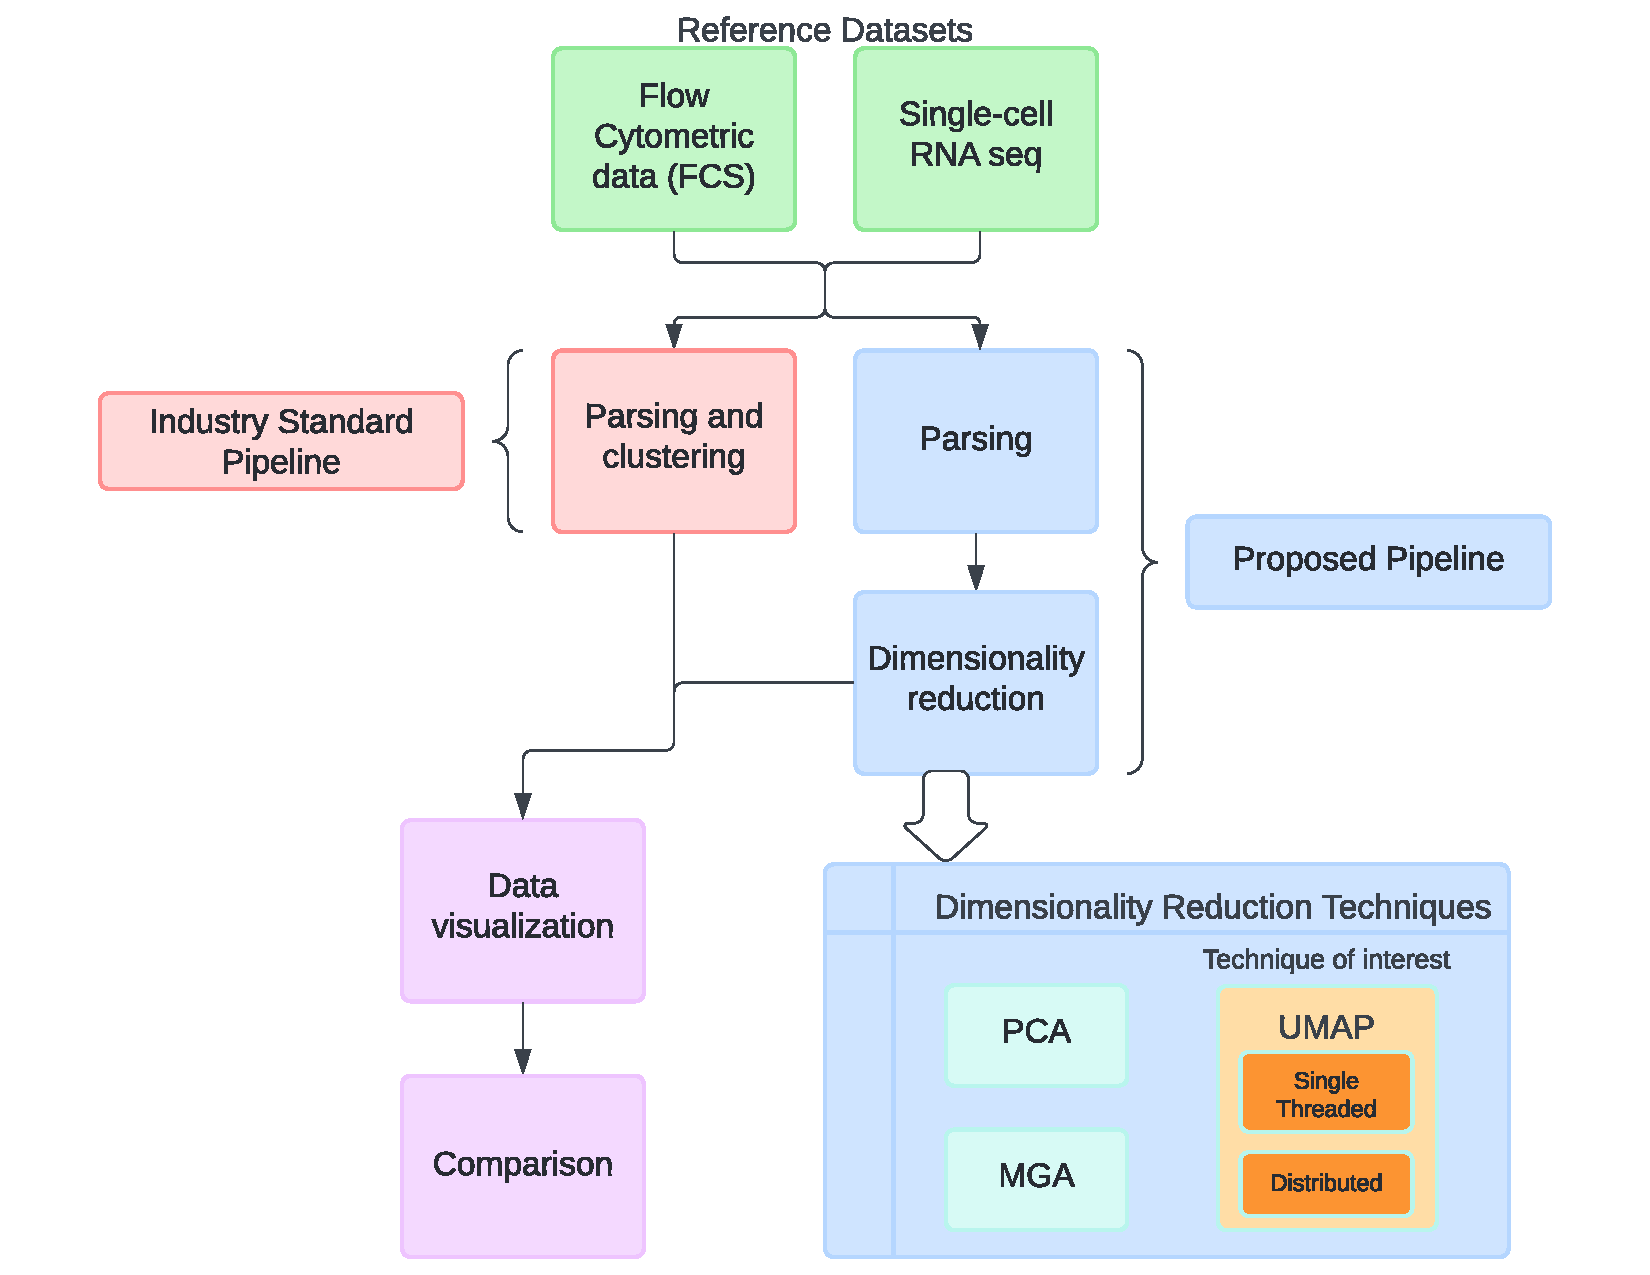
\includegraphics[width=3in]{whpc_data_diagram}
    \caption{Data will originate from 3rd-party reference datasets, be analyzed by our pipeline and a reference pipeline, and then our result will be compared against the reference for accuracy.}
    \label{fig:datadiagram}
  \end{minipage}
  % \begin{minipage}[b]{0.48\linewidth}
  %   \centering
  %   \begin{tabular}[l]{|l l|}
  %     \hline
  %     Resource & Quantity \\
  %     \hline
  %     CPUs & $\geq 2$ \\
  %     GPUs & 2 \\
  %     Storage & 2 TB \\
  %     \hline
  %   \end{tabular}\\
  %   \caption{Resource requirements}
  %   % \parbox{1.5in}{\captionof{table:resources}{Resource requirements}}
  %   \label{table:resources}
  % \end{minipage}
\end{figure}


\newgeometry{}
\printbibliography
\end{document}
